% По умолчанию используется шрифт 14 размера. Если нужен 12-й шрифт, уберите опцию [14pt]
\documentclass[russian,14pt]{matmex-diploma-custom}
\usepackage[table]{xcolor}
\usepackage{graphicx}
\usepackage{tabularx}
\newcolumntype{Y}{>{\centering\arraybackslash}X}
\usepackage{amsmath}
\usepackage{amsthm}
\usepackage{amsfonts}
\usepackage{amssymb}
\usepackage{mathtools}
\usepackage{thmtools}
\usepackage{thm-restate}
\usepackage{tikz}
\usepackage{wrapfig}
% \usepackage[kpsewhich,newfloat]{minted}
% \usemintedstyle{vs}
\usepackage[inline]{enumitem}
\usepackage{subcaption}
\usepackage{caption}
\usepackage[nocompress]{cite}
\usepackage{makecell}
% \setitemize{noitemsep,topsep=0pt,parsep=0pt,partopsep=0pt}
% \setenumerate{noitemsep,topsep=0pt,parsep=0pt,partopsep=0pt}
\graphicspath{ {resources/} }
% 
% % \documentclass 
% %   [ a4paper        % (Predefined, but who knows...)
% %   , draft,         % Show bad things.
% %   , 12pt           % Font size.
% %   , pagesize,      % Writes the paper size at special areas in DVI or
% %                    % PDF file. Recommended for use.
% %   , parskip=half   % Paragraphs: noindent + gap.
% %   , numbers=enddot % Pointed numbers.
% %   , BCOR=5mm       % Binding size correction.
% %   , submission
% %   , copyright
% %   , creativecommons 
% %   ]{eptcs}
% % \providecommand{\event}{ML 2018}  % Name of the event you are submitting to
% % \usepackage{breakurl}             % Not needed if you use pdflatex only.
% 
% \usepackage{underscore}           % Only needed if you use pdflatex.
% 
% \usepackage{booktabs}
% \usepackage{amssymb}
% \usepackage{amsmath}
% \usepackage{mathrsfs}
% \usepackage{mathtools}
% \usepackage{multirow}
% \usepackage{indentfirst}
% \usepackage{verbatim}
% \usepackage{amsmath, amssymb}
% \usepackage{graphicx}
% \usepackage{xcolor}
% \usepackage{url}
% \usepackage{stmaryrd}
% \usepackage{xspace}
% \usepackage{comment}
% \usepackage{wrapfig}
% \usepackage[caption=false]{subfig}
% \usepackage{placeins}
% \usepackage{tabularx}
% \usepackage{ragged2e}
% \usepackage{soul}
\usepackage{csquotes}
% \usepackage{inconsolata}
% 
% \usepackage{polyglossia}   % Babel replacement for XeTeX
%   \setdefaultlanguage[spelling=modern]{russian}
%   \setotherlanguage{english}
% \usepackage{fontspec}    % Provides an automatic and unified interface 
%                          % for loading fonts.
% \usepackage{xunicode}    % Generate Unicode chars from accented glyphs.
% \usepackage{xltxtra}     % "Extras" for LaTeX users of XeTeX.
% \usepackage{xecyr}       % Help with Russian.
% 
% %% Fonts
% \defaultfontfeatures{Mapping=tex-text}
% \setmainfont{CMU Serif}
% \setsansfont{CMU Sans Serif}
% \setmonofont{CMU Typewriter Text}

\usepackage[final]{listings}

\lstdefinelanguage{ocaml}{
keywords={@type, function, fun, let, in, match, with, when, class, type,
nonrec, object, method, of, rec, repeat, until, while, not, do, done, as, val, inherit, and,
new, module, sig, deriving, datatype, struct, if, then, else, open, private, virtual, include, success, failure,
lazy, assert, true, false, end},
sensitive=true,
commentstyle=\small\itshape\ttfamily,
keywordstyle=\ttfamily\bfseries, %\underbar,
identifierstyle=\ttfamily,
basewidth={0.5em,0.5em},
columns=fixed,
fontadjust=true,
literate={->}{{$\to$}}3 {===}{{$\equiv$}}1 {=/=}{{$\not\equiv$}}1 {|>}{{$\triangleright$}}3 {\\/}{{$\vee$}}2 {/\\}{{$\wedge$}}2 {>=}{{$\ge$}}1 {<=}{{$\le$}} 1,
morecomment=[s]{(*}{*)}
}

\lstset{
mathescape=true,
%basicstyle=\small,
identifierstyle=\ttfamily,
keywordstyle=\bfseries,
commentstyle=\scriptsize\rmfamily,
basewidth={0.5em,0.5em},
fontadjust=true,
language=ocaml
}
 
\newcommand{\cd}[1]{\texttt{#1}}
\newcommand{\inbr}[1]{\left<#1\right>}


\newcolumntype{L}[1]{>{\raggedright\let\newline\\\arraybackslash\hspace{0pt}}m{#1}}
\newcolumntype{C}[1]{>{\centering\let\newline\\\arraybackslash\hspace{0pt}}m{#1}}
\newcolumntype{R}[1]{>{\raggedleft\let\newline\\\arraybackslash\hspace{0pt}}m{#1}}



\usepackage{soul}
\usepackage[normalem]{ulem}
%\sout{Hello World}

% перевод заголовков в листингах
\renewcommand\lstlistingname{Листинг}
\renewcommand\lstlistlistingname{Листинги}


\usepackage{caption}
\usepackage{listings}

\DeclareCaptionFont{white}{ \color{white} }
\DeclareCaptionFormat{listing}{
    \parbox{\textwidth}{\hspace{15pt}#1#2#3}
}
\captionsetup[lstlisting]{ format=listing
  %, labelfont=white, textfont=white
  , singlelinecheck=false, margin=0pt, font={bf}
}

\graphicspath{ {images/} }

\begin{document}
%% Если что-то забыли, при компиляции будут ошибки Undefined control sequence \my@title@<что забыли>@ru
%% Если англоязычная титульная страница не нужна, то ее можно просто удалить.
\filltitle{ru}{
    %%
    chair              = {Математическое обеспечение и администрирование информационных систем},
    %% Макрос filltitle ненавидит пустые строки, поэтому обязателен хотя бы символ комментария на строке
    %% Актуально всем.
    title              = {Использование латентного пространства генеративных нейронных сетей для семантического редактирования фотографий},
    % 
    %% Здесь указывается тип работы. Возможные значения:
    type               = {master},
    author             = {Сугоняев Андрей Дмитриевич},
    % 
    %% Актуально только для ВКР. Указывается код и название направления подготовки.
    %% Те, что с 03 в середине --- бакалавриат, с 04 --- магистратура.
    specialty          = {02.04.03 <<Математическое обеспечение и администрирование информационных систем>>},
    % 
    %% Актуально только для ВКР. Указывается шифр и название образовательной программы.
    %%   ВМ.5665.2019 <<Математическое обеспечение и администрирование информационных систем>>
    %% Шифр и название программы можно посмотреть в учебном плане, по которому вы учитесь. 
    %% СВ.* --- бакалавриат, ВМ.* --- магистратура. В конце --- год поступления (не обязательно ваш, если вы были в академе/вылетали).
    programme          = {ВМ.5006.2019 <<Математическое обеспечение и администрирование информационных систем>>},
    %
    supervisorPosition = {д.ф.-м.н., профессор}, % Терехов А.Н.
    supervisor         = {А.Н. Терехов},  
    % 
    consultantPosition = {генеральный директор ООО <<СКЗ>>},
    consultant         = {А.А. Пименов},
    %
    %reviewerPosition   = {должность ООО <<Место работы>> степень},
    reviewerPosition   = {главный специалист ООО <<СКЗ>>, к.т.н.},
    reviewer           = {С.И. Федоренко},
}

\filltitle{en}{
    chair              = {Software and Administration of Information Systems},
    title              = {Using latent space of generative adversarial network for semantic photo editing},
    type               = {master},
    author             = {Andrey Sugonyaev},
    % 
    specialty          = {02.04.03 ``Software and Administration of Information Systems''},
    % 
    programme          = {ВМ.5006.2017 ``Software and Administration of Information Systems''},
    %
    % 
    %% Note that common title translations are:
    %%   кандидат наук --- C.Sc. (NOT Ph.D.)
    %%   доктор ... наук --- Sc.D.
    %%   доцент --- docent (NOT assistant/associate prof.)
    %%   профессор --- prof.
    supervisorPosition = {Sc.D., prof.},
    supervisor         = {A.N. Terekhov},
    % 
    consultantPosition = {CEO ``CVS''},
    consultant         = {A.A. Pimenov},
    %
    %reviewerPosition   = {position at ``Company'', degree if present},
    reviewerPosition   = {Chief Specialist ``CVS'', C.Sc.},
    reviewer           = {S.I. Fedorenko},
}
\maketitle
\setcounter{tocdepth}{2}
\tableofcontents

\section*{Введение}
Огромное количество информации об окружающем мире человек воспринимает интуитивно.

Несмотря на успехи в машинном и глубоком обучении, дискриминативные модели, т.е. модели, которые по наблюдаемым данным могут предсказать какую-то метку класса или какое-то значение, не могут понять сами данные. А потому эта информация им недоступна.

“Я не понимаю то, что я не могу воссоздать” — эта известная цитата Ричарда Фейнмана отражает основную идею генеративных моделей \cite{jebara2012machine}. Эти модели пытаются смоделировать данные, которые они наблюдают.

На сегодняшний день волну развития в области генеративных моделей возглавляют генеративные состязательные сети \cite{goodfellow2014generative}. Они представляют собой две нейронные сети, которые обучаются в тандеме: первая по входному случайному вектору учится генерировать изображение, вторая по сгенерированному изображению учится определять — реальное оно или нет?

Особенно большие успехи были достигнуты генеративными состязательными сетями в задаче генерации изображений лиц [progressive-gan, stylegan, stylegan2]. Эта задача обладает особой теоретической важностью, т.к. человеческий мозг способен интуитивно распознавать лица с малых лет и замечает их малейшие вариации и неточности.

Существующие генеративные состязательные сети способны генерировать реалистичные изображения лиц высокого разрешения, т.к. они обучились эффективно кодировать скрытую структуру изображений в своих внутренних представлениях.
Можно предположить, что генеративные состязательные сети также будут хорошо справляться с задачей семантического редактирования изображений, т.е. редактирования изображений в терминах признаков лиц, которые интуитивно понятны человеку.
Тем не менее, у подходов, которые напрямую обучают генеративные состязательные сети для решения этой задачи есть существенные недостатки.

В данной работе предлагается решить задачу семантического редактирования, взяв в качестве основы предобученную генеративную состязательную сеть для генерации лиц, и модифицировав ее архитектуру для предоставления возможности манипулировать ее внутренними представлениями.

\section*{Постановка задачи}
\label{sec:task}
% !TeX spellcheck = ru_RU
Целью данной работы является разработка и реализация решения для семантического редактирования изображений лиц на основе генеративных состязательные сетей. 
Решение должно быть способно определить то, как семантическая информация о лицевых признаках закодирована в латентном пространстве генеративной состязательной сети, обученной для генерации изображений лиц, и использовать эту информацию для манипулирования данными признаками.

Для достижения цели были поставлены следующие задачи:

\begin{enumerate}
\item провести обзор существующих архитектур генеративных состязательных сетей, предназначенных для генерации изображений лиц, а также существующих алгоритмов выделения семантики изображения;
\item разработать архитектуру решения для семантического редактирования изображений  на основе состязательных генеративных сетей;
\item реализовать прототип решения;
\item произвести эксперименты для качественной и количественной оценки полученного решения.
\end{enumerate}


\section{Обзор}
% !TeX spellcheck = ru_RU

\subsection{Генеративные состязательные сети}

Генеративные состязательные сети (\emph{Generative adversarial network}, сокр., \emph{GAN})  это семейство генеративных моделей, разработанное Яном Гудфеллоу в 2014 году \cite{goodfellow2014generative}.  Они формулируют процесс обучения  генеративной модели в виде антагонистической игры между двумя игроками: \emph{генератором} и \emph{дискриминатором}.

Генератор $G$ представляет собой глубокую нейронную сеть, задающую отбражение из латентного пространства $\mathcal Z$ в пространство данных $\mathcal X$.
Принимая на вход случайные вектора из некоторого заданного распределения $p(z)$ в $\mathcal Z$, он производит набор синтетических данных, пытаясь аппроксимировать распределение обучающей выборки $q_{data}(x)$.

% ... возвращает вероятность ...
Дискриминатор $D$ представляет собой глубокую нейронную сеть, задающую отбражение из пространства данных $\mathcal X$ в $\mathbb R$. Получив на вход некоторый элемент из пространства $\mathcal X$, дискриминатор возвращает значение, характеризующее вероятность того, что он был получен из распределения реальных данных $q_{data}(x)$, а не сгенерирован генератором $G$.

\begin{figure}[h]
\begin{center}
    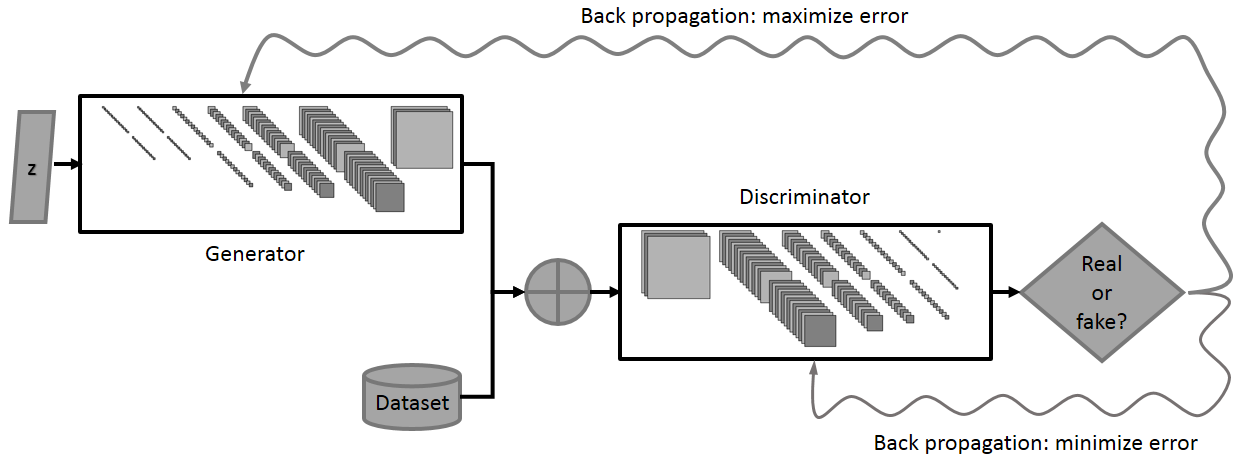
\includegraphics[width=0.9\textwidth]{gan}
    \caption{Архитектура генеративной состязательной сети.}
    \label{fig:subim11}
\end{center}
\end{figure}
% img src: https://blogs.nvidia.com/blog/2018/08/02/supervised-unsupervised-learning./

Роль дискриминатора состоит в том, чтобы как можно более точно отличать синтетические данные, полученные генератором, от реальных данный, взятых из обучающей выборки, в то время как генератор пытается обмануть дискриминатор путем генерирования синтетических данных, как можно более похожих на реальные.
Процесс совместного конкурентного обучения продолжается вплоть до достижения парой $(G, D)$ <<седловой точки>> (т.е. равновесия по Нэшу) \cite{goodfellow2017nips} функции выигрыша
$$
\min_{G} \max_{D} V(G, D) = \mathop{\mathbb{E}}_{x \sim q_{data}(x)} [\log D(x)] + \mathop{\mathbb{E}}_{z \sim p(z)} [\log (1 - D(G(z)))] ,
$$
в которой генератор способен генерировать данные, неотличимые дискриминатором от реальных.

\subsection{Генеративные нейронные сети для генерации лиц}

При решении задачи генерации изображений (в.т.ч. изображений лиц), пространство данных $\mathcal X$ предстваляет собой пространство изображений, каждый элемент которого обладает некоторым набором семантических признаков.
В случае лиц такими признаками могут являться положение головы, пол, возраст и т.д.

% семплированный -> взятый
Генератор $G$ является сверточной нейронной сетью, которая представляет собой композицию из $L$ сверточных слоев $G_1 ... G_L$ . 
Первый слой получает на вход случайный вектор $\mathbf z$, семплированный из многомерного нормального распределения $p(z)$ в латентном пространстве $\mathcal Z$, и возвращает тензор признаков $y_1 = G_1(\mathbf z)$. 
Каждый последующие слои применяется к выходам предыдущего: 
$$ y_i = G_i(y_{i-1}), $$
результатом применения последнего слоя является изображение $I = G_L(y_{L-1}) \equiv G(\mathbf z)$.

\subsubsection{BigGAN}
% TODO: абзац про то, что генерирование изобр. высокого разрешения - сложно

BigGAN \cite{bigGAN} --- генеративная состязательная сеть, спроектированная с целью масштабирования архитектуры для генерации изображений высокого разрешения.
BigGAN вносит ряд модификаций в стандартную архитектуру генеративных состязательных сетей.
Так, в архитектуру внедряются Skip\emph{-z} соединения, который позволяют промежучтоным слоям сети также принимать на вход латентный вектор:
$$ y_i = G_i(y_{i-1}, \mathbf z). $$
Кроме того, в архитектуре BigGAN применяются self-attention слой и спектральная нормализация весов.
Это позволяет увеличить количество весов модели в 2 раза и добиться качественной генерации изображений с разрешением до $512\times512$ на самых разнообразных классах изображений.

\subsubsection{StyleGAN}
StyleGAN \cite{StyleGAN} --– это генеративная состязательная сеть, архитектура которой разрабатывалась специально с целью генерации реалистичных изображений лиц.

% FIXME: linebreak
StyleGAN вводит промежуточное латентное пространство $\mathcal W$, предназначенное для решения проблемы кривизны, или "запутaнности" \linebreak (\emph{entanglement}), латентного пространства \cite{arvanitidis2018oddity}. 
Эта проблема возникает из-за ограничений и дефектов в вероятносном распределении тренировочных данных (рис. \ref{fig:stylegan-mapping}). 
Во время обучения StyleGAN выучивает нелинейное преобразование $M: \mathcal Z \mapsto \mathcal W$, которое позволяет избавиться от ограничений, накладываемых вероятносным распределением тренировочных данных, и получить более линейное латентное пространство.

\begin{figure}[h]
\begin{center}
    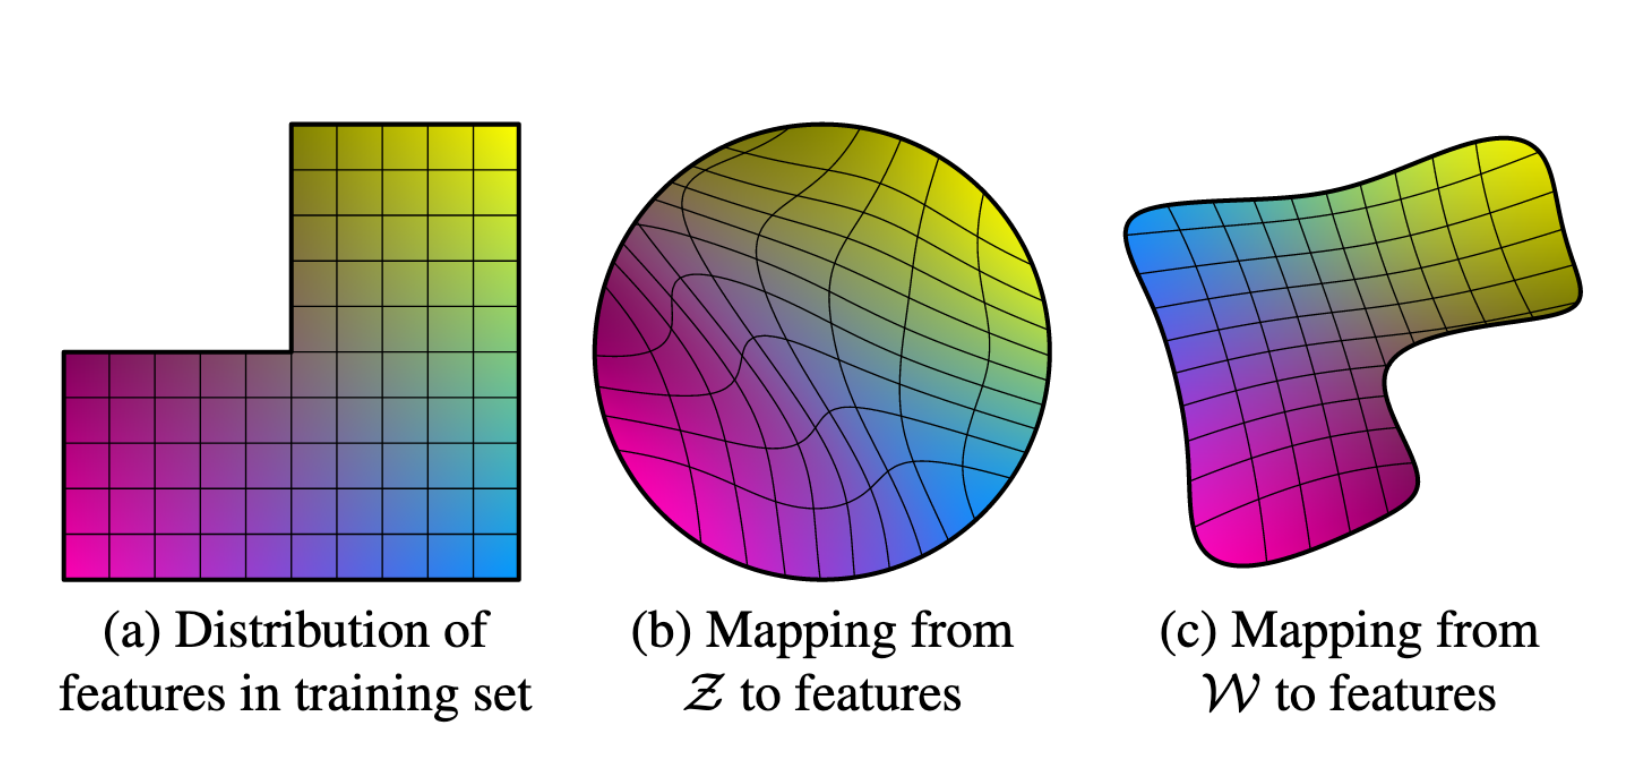
\includegraphics[width=0.7\textwidth]{stylegan_mapping}
    \caption{Иллюстрация действия промежуточного латентного пространства на примере двух факторов вариации (напр., \emph{пол} и \emph{наличие бороды}). Изображение взято из \cite{StyleGAN}.}
    \label{fig:stylegan-mapping}
    
    %FIXME: \small может лучше смотреться
    \footnotesize
 {(a)}~--- пример тренировочных данных, в которых отсутствует некоторая комбинация признаков; 
 {(b)}~--- это приводит к возникновению искривления отображения из $\mathcal Z$ в пространство признаков, которое исключает семплинг несуществующей комбинации из $\mathcal Z$;
 {(c)}~--- выучиваемое отображение из $\mathcal Z$ в $\mathcal W$ способно обратить данное искривление.

\end{center}
\end{figure}

StyleGAN модифицирует архитектуру генератора, основываясь на идеях из области Style Transfer. 
Синтез изображения начинается с фиксированного вектора $y_0$, а информация о латентном представлениии последовательно встраивается в каждый промежуточный слой генератора:
$$ y_i = G(y_{i-1}, \mathbf w),\quad \mathbf w = M(\mathbf z). $$
Это позволяет контролировать силу проявления различных семантических признаков изображения на разных масштабах, от грубых признаков, определяемых первыми слоями генератора, до тонких деталей, определяемых последними слоями.
В сочитании с встраиванием шума напрямую в слои сети, такая архитектура позволяет отделить высокоуровневые признаки изображения (положения лица, личность человека) от случайных вариационных факторов (волосы, веснушки и т.п.).

Кроме того, использование в каждом слое сети своего отдельного $\mathbf w_i$ позволяет производить операцию "смешивания стиля", комбинируя семантические признаки различных уровней абстракции с нескольких генерируемых изображений.

%TODO: как-то привести в именительный падеж
Дальнейшему улучшению данной архитектуры, StyleGAN2 \cite{karras2020stylegan2}, удалось добиться еще лучших результатов в задаче устранения "запутанности" латентного пространства и улучшения качества генерируемых изображений.
Кроме того, данной архитектурой также реализован алгоритм обратного отображения, названный StyleGAN2 Projector, который позволяет отобразить реальное изображение в латентное пространство сети.

\subsubsection{ALAE}
ALAE \cite{ALAE} –-- это генеративная нейронная сеть, архитектура которой разрабатывалась с целью предоставления возможности манипулирования латентными представлениями сети.

ALAE заимствует идеи вариационных автоэнкодеров \cite{kingma2014vae}, и дополняет стандартную архитектуру генеративных состязательных сетей энкодером $E$ и декодером $F$.
Декодер отображает входной латентный вектор в промежуточное латентное пространство $\mathcal W$, перед тем как подать его на вход генератору.
Энкодер отображает сгенерированное генератором изображение в промежуточное латентное пространство, перед тем как подать его на вход дискриминатору (рис. \ref{fig:alae}).

\begin{figure}[h]
\begin{center}
    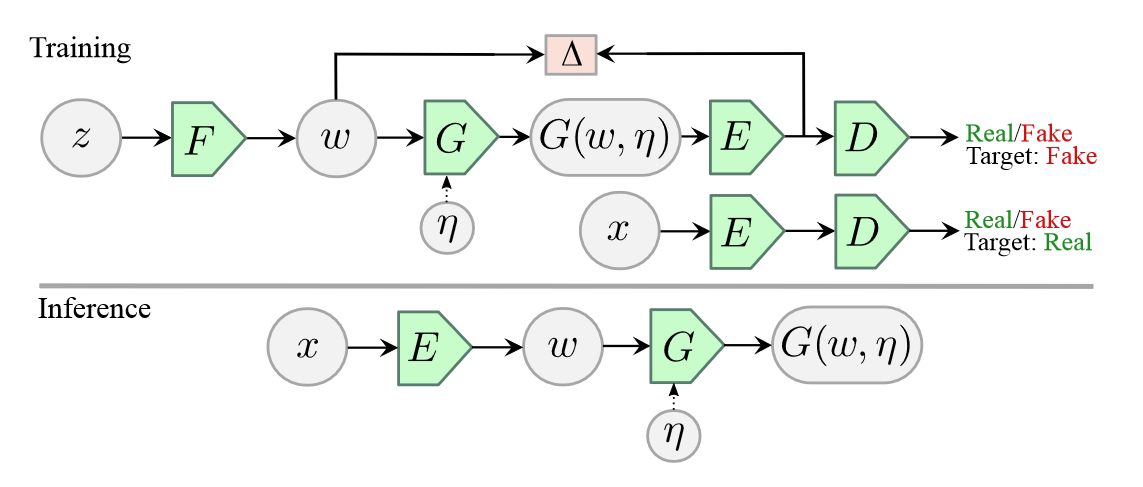
\includegraphics[width=0.9\textwidth]{ALAE}
    \caption{Архитектура ALAE. Изображение взято из \cite{ALAE}.}
    \label{fig:alae}
\end{center}
\end{figure}

В процессе обучения данная сеть применяет стратегию обучения автоэнкодеров, чтобы получить оптимальное латентное распределение в промежуточном латентном пространстве, накладывая ограничение о взаимной близости представлений, полученных энкодером и декодером;
и состязательную стратегию обучения, чтобы аппроксимировать распределение данных обучающей выборки.


\subsection{Алгоритмы отображения изображений в латентное пространство сети}

Для работы с реальными изображениями генеративным состязательным сетям требуется обратное отображение, позволяющее по входному изображению получить соответствующий ему латентный вектор в латентном пространстве сети. 
Классическая архитектура генеративных состязательных сетей не задает такого отображения напрямую, а потому для работы с реальными изображениями реализуются алгоритмы, позволяющие аппроксимировать данный латентный вектор.

Обучение дополнительного энкодера \cite{donahue2016adversarial} является распространенным подходом к нахождению обратного отображения.
Обратное отображение аппроксимируется нейронной сетью, которая обучается решению задачи регрессии латентного вектора по заданному входному изображению. 
Обучение энкодера производится на датасете пар <\emph{изображение, вектор}>, состоящем из набора синтетических изображений, сгенерированных генеративной состязательной сетью, и входных латентных векторов, с помощью которых это изображение было получено.

Латентная оптимизация \cite{perarnau2016invertible} --- это алгоритм приближения латентного вектора путем минимизации некоторой заданной функции потерь реконструкции.
Алгоритм определяет некоторую гладкую функцию потерь $loss(I_{real}, G(\mathbf z)) $, которая характеризует, насколько изображение, сгенерированное с помощью текщего латентного вектора $\mathbf z$, близко к входному изображению $I_{real}$.
Поскольку генератор $G(z)$ является отображением, дифференциируемым по входному вектору (благодаря методу обратного распространения ошибки), а его гладкость зависит главным образом от выбора гладких функций активации (т.к. он является композицией линейных слоев и функций активации), это позволяет минимизировать заданную функцию потерь методом градиентного спуска, итеративно обновляя латентный вектор.

Использование в качестве архитектуры генератора StyleGAN позволяет улучшить процесс латентной оптимизации.
Оптимизация в расширенном латентном пространстве $\mathcal W+$, которое представляет собой конкатенацию 18 различных векторов $\mathbf w_i$, поступающих на вход каждому отдельному слою архитектуры StyleGAN, позволяет получить более точную реконструкцию входного изображения \cite{abdal2019image2stylegan}.


\subsection{Алгоритмы выделения семантик изображения в латентном пространстве сети}

Идея манипулирования латентным вектором для изменения семантических признаков генерируемых изображений основана на наблюдении о том, что к латентным векторам применима векторная арифметика \cite{radford2015unsupervised}.

Многие исследования латентных пространств генеративных состязательных сетей исходят их предположения о том, что отдельные факторы вариации генерируемых изображений контролируются некоторыми одномерными линейными подпространствами латентного пространства сети \cite{StyleGAN}.
Таким образом, зная базисный вектор подпространства, соответствующего определенному семантическому признаку, можно добиться увеличения или уменьшения выраженности данного признака на сгенерированном изображении путем линейного сдвига латентного вектора в направлении данного базисного вектора \cite{abdal2019image2stylegan}. 
Далее данный вектор будем называть \emph{семантическим вектором признака} в латентном пространстве генеративной состязательной сети.

GANSpace \cite{hrknen2020ganspace} --- это фреймворк, предназначенный для выделения и анализа семантических векторов, и использования их для редактирования семантических признаков на генерируемом изображении.
Для выделения семантических векторов данным фреймворком реализуется алгоритм, базирующийся на методе главных компонент.
Он применяет метод главных компонент для уменьшения размерности латентного пространства и выделения в нем наиболее значимых направлений. Эти направления принимаются в качестве базисных векторов, и дальнейший визуальный анализ изменений, которые вызывает линейный сдвиг по данным направлениям на генерируемых изображениях, показывает, каким семантическим признакам эти направления соответствуют.

InterFaceGAN \cite{shen2020interfacegan} --- это фреймворк, нацеленный на более контролируемое исследование латентного пространства генеративной состязательной сети.
Он ставит своей задачей нахождение того, как в латентное пространство отображается некоторый бинарный семантический признак, заданный набором пооложительных и отрицательных примеров.
Для этого фреймворком InterFaceGAN реализуется одноименный алгоритм выделения семантических векторов.
Этот алгоритм базируется на обозначенном в \cite{StyleGAN} факте о том, что два набора латентных векторов, соответствующих изображениям с различными значениями некоторого бинарного семантического признака, будут линейно разделимы в латентном пространстве.
Нахождение семантического вектора заданного бинарного признака сводится к нахождению оптимальной разделяющей гиперплоскости между данными наборами латентных векторов.
В качестве семантического вектора берется нормальный вектор найденной гиперплоскости.


\section{Алгоритм выделения линейных подпространств, соответствующих семантикам изображения}
\emph{Здесь будет расписан алгоритм выделения семантик, лежащий в основе решения.}

Для выделения семантик изображения принимается предположение о линейности латентного пространства.

Рассмотрим произвольный бинарный признак, заданный дискриминативной функцией $f : \mathcal X \mapsto \{0,1\}$, определяющей наличие или отсутствие этого признака на изображении.
При справедливости этого предположения линейная интерполяция между двумя латентными векторами, соответствующими двум изображениям, на одном из которых признак присутствует, а на другом --- отсутствует, приведет к постепенному и непрерывному изменению этого признака на генерируемом изображении. 

Как показано в \cite{StyleGAN}, линейная разделимость бинарных признаков в промежуточном латентном пространстве $\mathcal{W}$ позволяет найти векторы направлений, соответствующих отдельным факторам вариации, т.е. отдельным признакам.

Для нахождения данных направлений используется следующий метод.
\begin{itemize}
    \item В качестве функции $f$ используется нейросетевой классификатор, обученный на датасете CelebA-HQ. Архитектура крассификатора аналогична архитектуре дискриминатора, используемого в \cite{progressive-growing-gan, StyleGAN}. В качестве рассматриваемых признаков были выбраны \emph{наличие улыбки} и \emph{поворот головы}.
    \item С помощью имеющегося генератора $G$ генерируется набор данных, состоящий из $20000$ изображений. Данный набор размечается с помощью классификатора $f$.
    \item На полученном наборе данных обучается линейная SVM \cite{svm} и находится оптимальная разделяющая гиперплоскость. 
\end{itemize}
Нормальный вектор полученной гиперплоскости задает направление, соответствующее рассматриваемому признаку.
%\subsection{Генерация данных}
%\subsection{Оптимальная разделяющая гиперплоскость}
%\subsection{Линейная разделимость в латентном пространстве}

\begin{figure}[h]
\begin{center}
    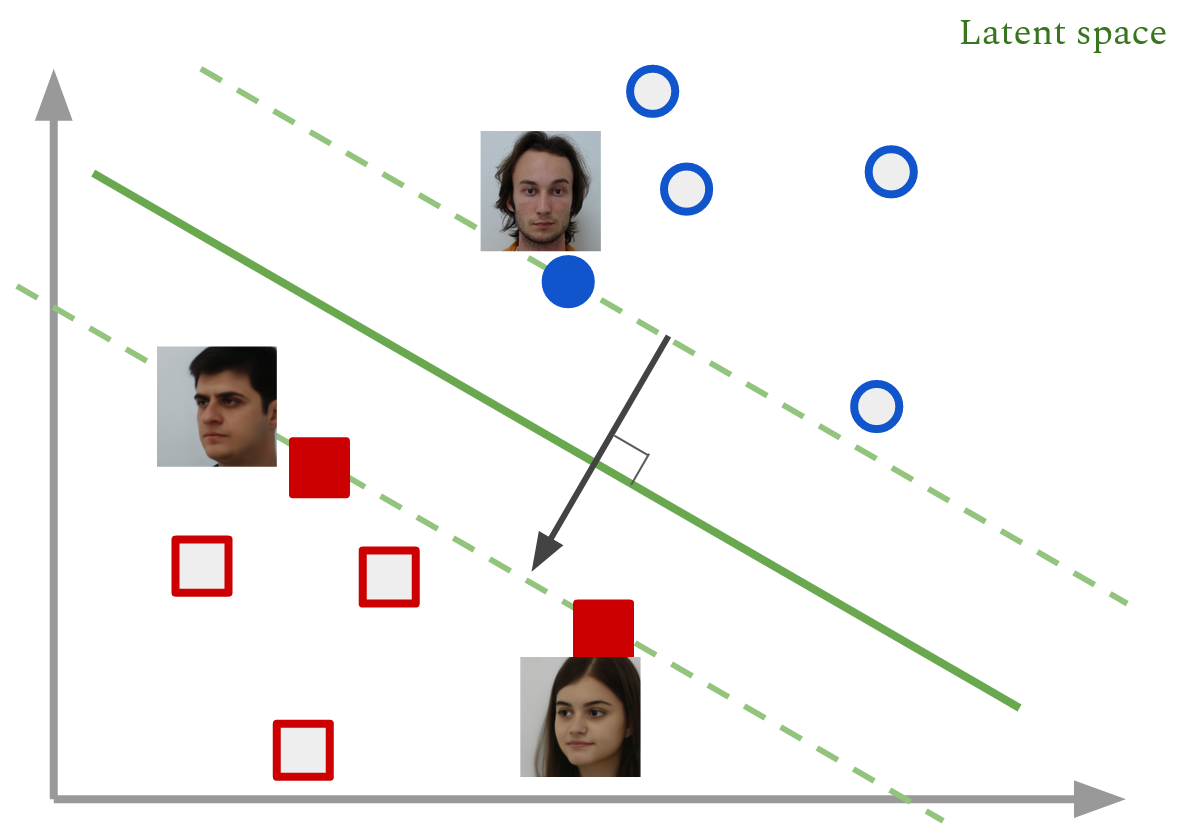
\includegraphics[width=0.7\textwidth]{boundary-SVM}
    \caption{Иллюстрация процесса нахождения векторов направлений, соответствующих отдельным факторам вариации, путем нахожения оптимальной разделяющей плоскости.}
    \label{fig:svm-boundary}
\end{center}
\end{figure}

\section{Архитектура решения}
\emph{Здесь расписывается архитектура.}

\begin{figure}[h]
\begin{center}
    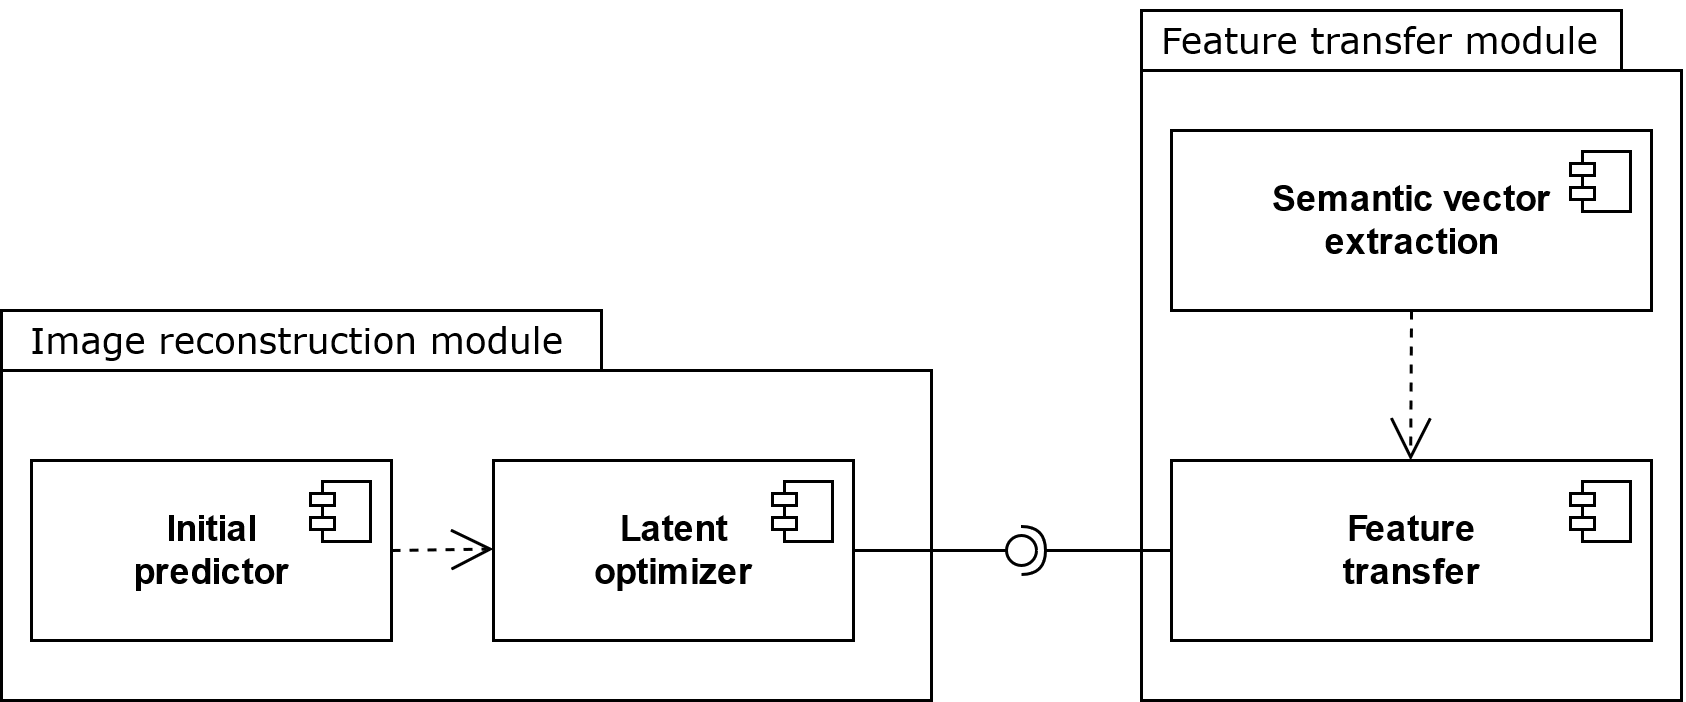
\includegraphics[width=0.9\textwidth]{Architecture_eng}
    \caption{Архитектура решения (\emph{Диаграмма в процессе работы, GAN-ы отдельно не надо, потому что композиция, и они часть компонента, в feature transfer добавить выделение фич}).}
    \label{fig:architecture}
\end{center}
\end{figure}

В рамках данной работы было разработано решение для семантического редактирования изображений. Это решение позволет редактировать изображения лиц в терминах высокоуровневых лицевых признаков, нитуитивно понятных человеку. %таких как положение головы, наличие улыбки и т.д.
% с двумя режимами работы: 1) по предоставленному методу разметки выделить семантический признак в латентном пространстве сети, 2) ...
По двум входным изображениям, целевому изображению и изображению-образцу, это решение способно произвести перенос заданного лицевого признака с изображения-образца на целевое изображение.
Решение способно работать с произвольными бинарными признаками, но ...
%Для неизвестного признака решение может что -то зделать, если передана процедура разметки/Чтобы добавить новый признак

Решение состоит из двух функциональных частей: модуля реконструкции изображения (?в латентном пространстве генеративной состязательной сети), и модуля семантического редактирования (?в латентном пространстве сети).

Первый модуль осуществляет отображение входных изображений в латентное пространство имеющейся генеративной состязательной сети, т.е. находит такой латентный вектор, с помощь которого генератор имеющейся генеративной состязательной сети сгенерирует максимально похожее изображение.
% он включает в себя компонент1 и компонент2 (?)
% он производит гибридный метод латентной оптимизации (отсылаемся к обзору), энкодер предсказывает начальное приближение, потом непосредственная оптимизация латентного вектора.
%Здесь пишем что это в.т.ч. для артист-контроля, позволяет быстро получить отклик для пользователя, и при этом дать гибкий контроль между затраченным временем и полученной точностью.

Второй модуль осуществляет манипулирование полученными латентными представлениями. Этот модуль отвечает за выявление преобразования в латентном пространстве, соответствующего заданному лицевому признаку, а также за процесс переноса заданного признака с изображения образца на целевое изображение.
% он включает в себя компонент3 и компонент4
% здесь пишем про то, что для выделения семантик нужна процедура разметки (или выборка положительных/отрицательных примеров), а также про то, что мы вводим нелинейность для сохранения личности?

%Оба модуля взаимодействуют с пользователем посредством веб—интерфейса.

\section{Особенности реализации}
\emph{Здесь описывается реализация, в.т.ч. гиперпараметры и процесс обучения доп. классификаторов.}

\subsection{Энкодер начального приближения латентной оптимизации}
%Возможно этот абзац стоит в переработанном виде кинуть в архитектуру!
Чтобы ускорить процесс сходимости латентной оптимизации, в данной работе предлагается использовать гибридный подход. Предлагается обучить дополнительную нейронную сеть-энкодер, которая по входному изображению даст грубое приближение его латентного вектора. Использование данное приближение в качестве начального приближения позволит ускорить роцесс сходимости.

Для предсказания начального приближения латентной оптимизации была обучена сверточная нейронная сеть ResNet.
%почему резнет

Для ее обучения с помощью имеющейся генеративной состязательной сети было сгенерированно $50000$ изображений и соответствующих им латентных векторов.
По входному изображению сеть ResNet обучалась предсказывать его латентный вектор. В качестве функции потерь использован логарифм гиперболического синуса ошибки (\emph{Log-Cosh Loss} \cite{chen2019log}), который является гладким аналогом средней абсолютной ошибки.
%log cosh loss, то что он хорош при обучении вариационных автокодировщиков

Нейронная сеть реализована на  фреймворке PyTorch. Сеть обучалать $20$ эпох методом обратного распространения ошибки с использованием оптимизационного алгоритма Adam.
%график нужен

\subsection{Нейронная сеть для латентной оптимизации}

Генератор $G$ является дифференциируемой по входам нейронной сетью, что позволяет напрямую оптимизировать латентный вектор, минимизируя функцию потерь реконструкции. Этот процесс называется латентной оптимизацией. 

\emph{Нужно поправить обозначения на изображении.}
\begin{figure}[h]
\begin{center}
    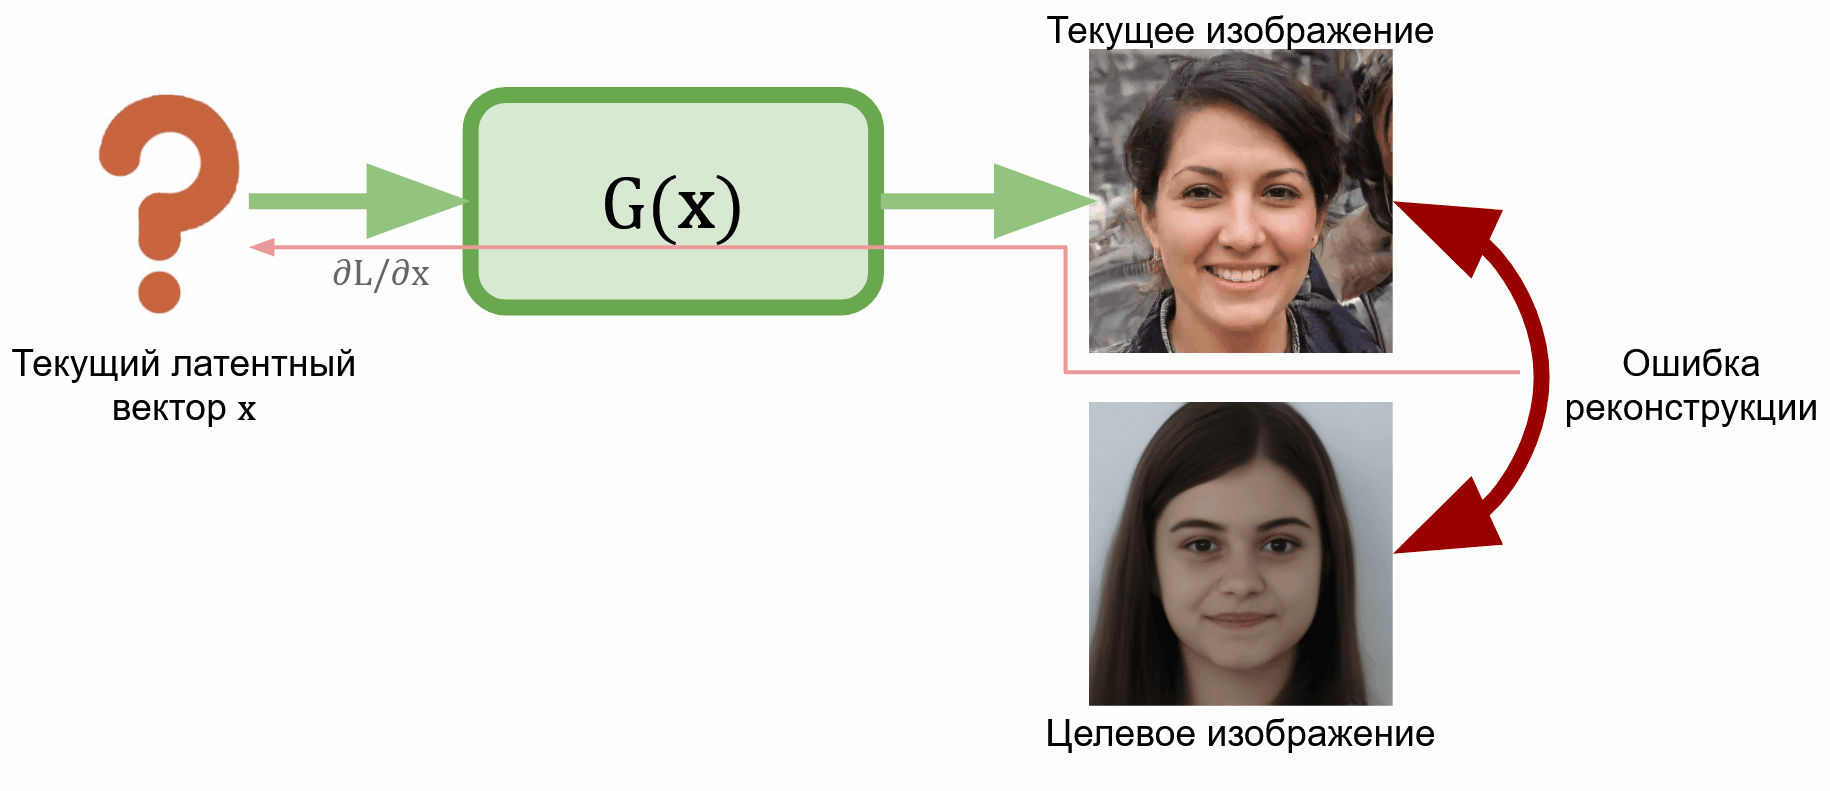
\includegraphics[width=0.9\textwidth]{optim_pipeline_ru}
    \caption{Архитектура нейронной сети для латентной оптимизации}
    \label{fig:optim_pipelin}
\end{center}
\end{figure}

В качестве функцию потерь реконструкции используется взвешенная сумма среднеквадратичной ошибки в пространстве пикселей и визуальной функции потерь (\emph{perceptual loss} \cite{Johnson2016Perceptual}).
%Здесь нужно сказать, что следуем Image2StyleGAN, что используем W+

\emph{Дальше нужно написать достаточно сложный абзац, объясняющий пространство $W+$ и оптимизацию отдельных грубых мап признаков.}
%собственно здесь описываем модификацию того, что ступенчато оптимизируемся и что это позволяет не улететь датеко от данных (см. Latent Space Oddity).


%\subsection{Алгоритм выделения семантик}
\subsection{Алгоритм выделения линейных подпространств, соответствующих семантикам изображения}
\emph{Здесь будет расписан алгоритм выделения семантик, лежащий в основе решения.}

Для выделения семантик изображения принимается предположение о линейности латентного пространства.

Рассмотрим произвольный бинарный признак, заданный дискриминативной функцией $f : \mathcal X \mapsto \{0,1\}$, определяющей наличие или отсутствие этого признака на изображении.
При справедливости этого предположения линейная интерполяция между двумя латентными векторами, соответствующими двум изображениям, на одном из которых признак присутствует, а на другом --- отсутствует, приведет к постепенному и непрерывному изменению этого признака на генерируемом изображении. 

Как показано в \cite{StyleGAN}, линейная разделимость бинарных признаков в промежуточном латентном пространстве $\mathcal{W}$ позволяет найти векторы направлений, соответствующих отдельным факторам вариации, т.е. отдельным признакам.

Для нахождения данных направлений используется следующий метод.
\begin{itemize}
    \item В качестве функции $f$ используется нейросетевой классификатор, обученный на датасете CelebA-HQ. Архитектура крассификатора аналогична архитектуре дискриминатора, используемого в \cite{progressive-growing-gan, StyleGAN}. В качестве рассматриваемых признаков были выбраны \emph{наличие улыбки} и \emph{поворот головы}.
    \item С помощью имеющегося генератора $G$ генерируется набор данных, состоящий из $20000$ изображений. Данный набор размечается с помощью классификатора $f$.
    \item На полученном наборе данных обучается линейная SVM \cite{svm} и находится оптимальная разделяющая гиперплоскость. 
\end{itemize}
Нормальный вектор полученной гиперплоскости задает направление, соответствующее рассматриваемому признаку.
%\subsection{Генерация данных}
%\subsection{Оптимальная разделяющая гиперплоскость}
%\subsection{Линейная разделимость в латентном пространстве}

\begin{figure}[h]
\begin{center}
    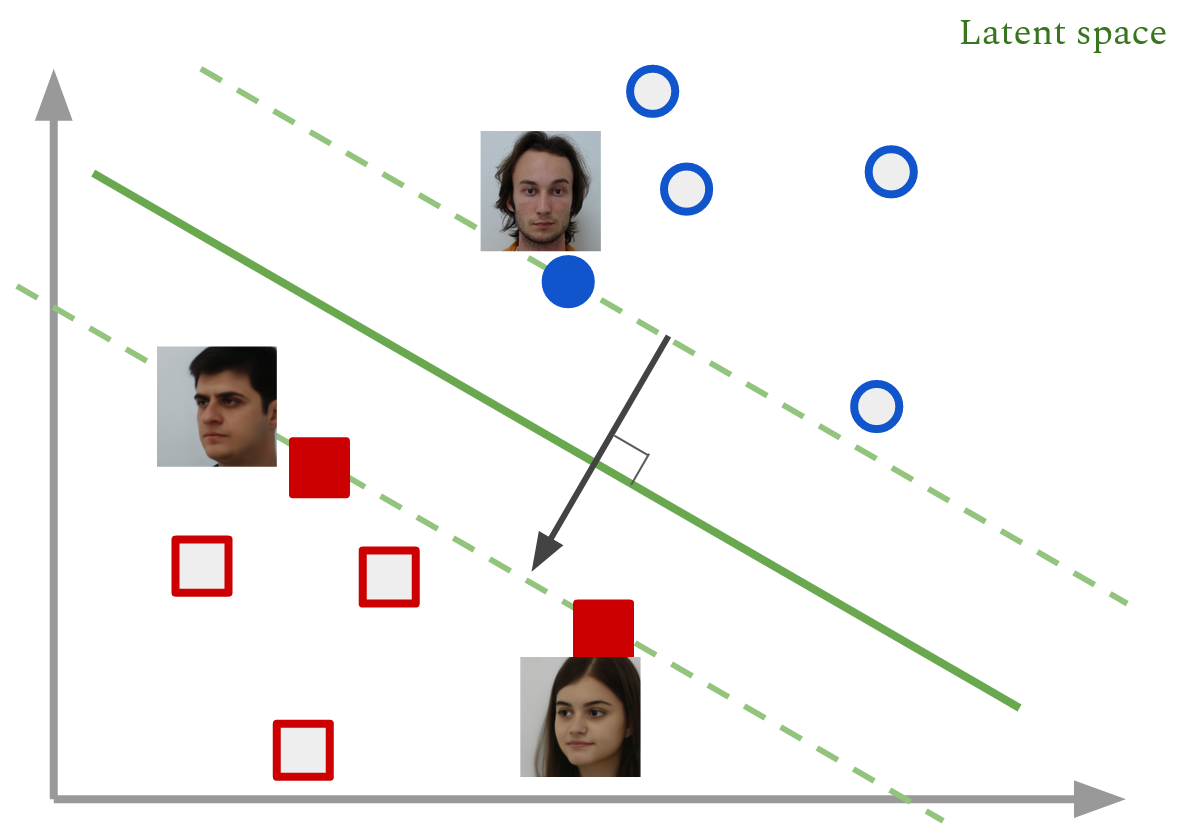
\includegraphics[width=0.7\textwidth]{boundary-SVM}
    \caption{Иллюстрация процесса нахождения векторов направлений, соответствующих отдельным факторам вариации, путем нахожения оптимальной разделяющей плоскости.}
    \label{fig:svm-boundary}
\end{center}
\end{figure}


\subsection{Алгоритм переноса лицевых признаков с изображения образца}

%Переформулировать в терминах оптимизации.

% Мы оптимизируем пока не сойдемся по одному Degree of Freedom, и при этом делаем ортогональный шаг по остальным Degree of Freedom.
На генерируемом изображении $g(\mathbf x + \alpha \mathbf n)$, полученном путем линейного сдвига в направлении полученного вектора $\mathbf n$, выбранный семантический признак будет более выражен при $\alpha > 0$, и менее выражен при $\alpha  < 0$.

%собственно здесь описываем модификацию того, что используется Face Model для введения нелинейности и сохранения личности.

\section{Эксперименты}
% !TeX spellcheck = ru_RU

Для количественной оценки результатов работы решения, а также сравнения с предложенных в решении алгоритмических модификаций с алгоритмами, указанными в главе \ref{sec:relatedworks}, был проведен ряд экспериментов.


\subsection{Задачи эксперимента}
В ходе экспериментов были исследованы следующие вопросы:

\textbf{RQ 1: } Насколько качественно производится реконструкция входных изображений в латентном пространстве генеративной состязательной сети с помощью примененного в решении алгоритма по сравнению с существующими state-of-the-art алгоритмами?

\textbf{RQ 2: }Насколько хорошо работает примененный в решении алгоритм переноса признаков по сравнению с существующими state-of-the-art алгоритмами?

%\begin{enumerate}
%    \item 
%    % Оценка качества реконструкции реальных изображений
%    Насколько качественно производится реконструкция входных изображений в латентном пространстве генеративной состязательной сети с помощью примененного в решении алгоритма по сравнению с существующими state-of-the-art алгоритмами?
%    \item 
%    % Оценка качества переноса лицевых признаков
%    Насколько хорошо работает примененный в решении алгоритм переноса признаков по сравнению с существующими state-of-the-art алгоритмами?
%\end{enumerate}


\subsection{Метрики}
% нужны ссылки.
Следуя мотивации, представленной в литературе по генеративным состязательным сетям, были использованы метрики FID, LPIPS, и Face identity score. Кроме того, в качестве сравниваемой метрики использовалось количество времени, затрачиваемое алгоритмом на обработку одного изображения.

\paragraph{FID.} 
Чтобы измерить реалистичность получаемых изображений применяется метрика FID (\emph{Frechet inception distance}) \cite{heusel2017fid}, используемая для измерения качества изображений, сгенерированных с помощью генеративной нейронной сети.
Эта метрика позволяет сравнить распределение сгенерированных изображений, полученных в результате применения оцениваемых алгоритмов, с распределением набора реальных изображений.

\paragraph{LPIPS.}
Для оценки схожести реальных входных изображений и сгенерированных изображений, полученных в результате работы алгоритма, применяется метрика визуальной схожести LPIPS \cite{zhang2018lpips}.

\paragraph{Face identity score.}
Для того, чтобы численно оценить меру сохранения лицевых признаков, которые определяют личность человека, между реальным входным изображением и изображением, реконструированным или отредактированным с помощью генеративной нейронной сети, применяется метрика Face identity score.
Для этого используется нейросетевая модель для распознавания лиц \cite{deng2018arcface}, с помощью которой по изображениям получаются векторные ембеддинги.
По паре изображений, а именно реальному изображению и его реконструкции, или изображению до и после редактирования, вычисляется мера косинусного сходства (\emph{cosine similarity}) между их эмбеддингами.


\subsection{Данные}
Эксперименты были проведены на двух датасетах: CelebA-HQ \cite{progressive-growing-gan} и FEI Face Database \cite{fei-database}.

Датасет CelebA-HQ --- это высококачественная версия набора изображений CelebA \cite{liu2015celeba}, которая содержит $30000$ изображений с расширением $1024\times1024$.
Этот датасет содержит изображения $10177$ различных знаменитостей, полученные путем предобработки и выравнивания реальных фотографий.
Кроме того, для каждого изображения отмечены координаты $5$ особых точек лица и значения $40$ бинарных лицевых признаков.

Датасет FEI Face Database представлет собой набор из $2800$ изображений, полученных в студийных условиях.
Он содержит по $14$ изображений на каждого из $200$ субъектов.
Каждый субъект представлен набором изображений, на которых варьируются такие лицевые признаки, как \emph{положение головы}, \emph{наличие улыбки} и \emph{освещение}.


\subsection{Методология экспериментов}
\paragraph{RQ 1:}
Сравнение качества реконструкции производится со следующими алгоритмами: StyleGAN2 Projector \cite{karras2020stylegan2} и энкодер, используемый в архитектуре ALAE \cite{ALAE}.
Для этого производится отображение изображений, взятых из датасета CelebA-HQ, в латентное пространство соответствующей модели.
Затем подсчитываются метрика реалистичности (FID) и метрики визуальной схожести (LPIPS, Face identity score) между реальным изображением и его реконструкцией.
Также подсчитывается время, затраченное алгоритмом на обработку одного изображения.
Результаты данного эксперимента представлены в Таблице \ref{tab:exp1}.

\begin{table}
\begin{center}
  \caption{Результаты эксперимента по оценке качества реконструкции изображений.}
  \label{tab:exp1}
  \begin{tabular}{ |r|c|c|c|c| } 
    \hline
      & FID ↓ & LPIPS ↓ & F.i.s. ↑ & Время ↓ \\ 
    \hline\hline
    ALAE    & 54.686 & 0.403 & 0.494 & \textbf{0.28s}  \\ 
    StyleGAN2 Projector 
            & \textbf{54.484} & 0.332 & 0.591 & 37.57s  \\ 
    Решение & 68.129 & \textbf{0.248} & \textbf{0.853} & 33.71s  \\ 
    \hline
  \end{tabular}
\end{center}
\end{table}

\paragraph{RQ 2:}
Сравнение качества переноса лицевых признаков производится со следующими алгоритмами: Image2StyleGAN \cite{abdal2019image2stylegan} и GANSpace \cite{hrknen2020ganspace}.
Для данного сравнения в качестве редактируемых признаков были выбраны \emph{положение головы} и \emph{наличие улыбки} на изображении.

Для проведения данного эксперимента изображения, взятые из датасета FEI Face Database, разбиваются на 3 набора: набор входных изображений, на которых отсутствует рассматриваемый признак, набор целевых изображений тех же субъектов, на которых присутствует рассматриваемый признак, и набор изображений-образцов, который не содержит субъектов, изображения которых взяты в качестве входных изображений, и на которых присутствует рассматриваемый признак.
Входные изображения и изображения-образцы отображаются в латентное пространство сети StyleGAN с использованием реализованного в данной работе алгоритма отображения.
Затем к входным изображениям применяется алгоритм переноса признака, котороый использует в качестве изображения-образца случайное изображение из набора изображений-образцов.

Между изображениями, полученными в результате применения алгоритма, и целевыми изображениями подсчитываются метрики визуальной схожести (LPIPS, Face identity score) а также метрика реалистичности (FID).
Также подсчитывается время, затраченное алгоритмом на обработку одного изображения.
Результаты данного эксперимента представлены в Таблице \ref{tab:exp2}.

\begin{table}
\begin{center}
  \caption{Результаты эксперимента по оценке качества переноса лицевых признаков.}
  \label{tab:exp2}
  \begin{tabular}{ |r c|c|c|c|c| } 
    \hline
      & & FID ↓ & LPIPS ↓ & F.i.s. ↑ & Время ↓ \\ 
    \hline\hline
    GANSpace & (\emph{pose}) & 166.630 & 0.352 & 0.582 & 0.344s \\
            & (\emph{smile}) & 147.160 & 0.276 & 0.748 &  \\
    \hline
    Image2StyleGAN 
             & (\emph{pose}) & 155.503 & 0.328 & 0.643 & \textbf{0.314s} \\
            & (\emph{smile}) & 120.609 & \textbf{0.239} & 0.769 & \\
    \hline
    Решение  & (\emph{pose}) & \textbf{148.053} & \textbf{0.319} & \textbf{0.695} & 38.25s \\ 
            & (\emph{smile}) & \textbf{117.021} & 0.241 & \textbf{0.784} &  \\ 
    \hline
  \end{tabular}
\end{center}
\end{table}

\subsection{Анализ результатов}

Как видно из результатов, представленных в табл. \ref{tab:exp1}, реализованный в данном решении алгоритм отображения изображений в латентное пространство генеративной состязательной сети демонстрирует улучшение метрик визуальной схожести LPIPS (на $0.084$) и Face identity score (на $0.262$).
Тем не менее, он демонстрирует ухудшение по метрике реалистичности FID (на $13.645$).
Кроме того, в данном решении удалось ускорить алгоритм латентной оптимазации по сравнению с StyleGAN2 Projector (на $3.86$ c). Несмотря на это, он не может конкурировать по времени работы с алгоритмом ALAE, использующим только энкодер.

Ухудшение метрики реалистичности FID может говорить о возникновении артефактов на генерируемом изображении, связанных с тем, что латентная оптимизация попадает в область латентного пространства, удаленную от распределения первоначальных тренировочных данных.
Поэтому используемая генеративная нейронная сеть испытывает трудности при генерации качественного изображения.
Кроме того, это также может говорить о том, что реализованный алгоритм латентной оптимизации подвержен застреванию в локальном минимуме. Для анализа и решения данной проблемы требуется дальнейшее исследование.

Результаты оценки реализованного в данном решении алгоритма переноса лицевых признаков, представленные в табл. \ref{tab:exp2}, демонстрируют улучшение как метрики реалистичности FID, так и метрик визуальной схожести LPIPS и Face identity score.
Стоит отметить, что более значимых улучшений удается добиться при редактированиии признака \emph{положение головы} (FID на $7.45$, LPIPS на $0.009$, Face identity score на $0.052$).

Тем не менее, реализованный алгоритм демонстрирует увеличение количества времени, затрачиваемого на обработру изображения.
Это связано с итеративной природой алгоритма переноса.
В отличие от алгоритмов GANSpace и Image2StyleGAN, которые единожды применяют линейный сдвиг в латентном пространстве генеративной состязательной сети, в реализованном алгоритме применяется пошаговая оптимизация, в которой на каждом шаге требуется сгенерировать изображение по текущему приближению и скорректировать его для сохранения семантических признаков, определяющих личность.

\section*{Заключение}
В рамках данной выпускной квалификационной работы разработано\footnote{https://github.com/Andre6o6/stylegan-editing} решение для редактирования лицевых признаков на изображении, использующее предобученную для генерации изображений лиц генеративную состязательную сеть.

В ходе работы были получены следующие результаты:

\begin{itemize}
\item Проведен обзор существующих архитектур генеративных состязательных сетей для генерации изображений лиц --- BigGAN, StyleGAN, ALAE --- и приведены доводы в пользу использования архитектуры StyleGAN в качестве основы для алгоритма.
\item Реализован алгоритм выделения линейных подпространств, соответствующих семантикам изображения, в латентном пространстве сети.
\item Разработана архитектура нейронной сети для отображения входного изображения в латентное пространство, позволяющая контролировать баланс между точностью реконструкции изображения и затраченным временем.
\item Разработан алгоритм переноса произвольного бинарного лицевого признака с изображения-образца на целевое изображение. 
\item Прототип решения реализован на языке Python с использованием фреймворка PyTorch.
\item Проведены эксперименты для оценки работы алгоритма. Результаты проведенных экспериментов показывают улучшение качества реконструкции реальных изображений по сравнению с существующими подходами --- StyleGAN2 Projector и ALAE. В эксперименте по реконструкции изображений из датасета FFHQ предложенное решение показывает улучшение метрик визуальной схожести LPIPS и Face Identity Score.
\item Также результаты проведенных экспериментов показывают улучшение переноса лицевых признаков по сравнению с существующими подходами --- Image2StyleGAN и GANSpace.  В эксперименте по переносу признаков на изображениях из датасета FEI Face Database предложенное решение показывает улучшение метрики реалистичности FID, а также LPIPS и Face Identity Score.
\end{itemize}

% \nocite{*}
\setmonofont[Mapping=tex-text]{CMU Typewriter Text}
\bibliographystyle{ugost2008ls}
\bibliography{vkr}
\end{document}
